\documentclass[tikz,border=12pt]{standalone}
\usepackage[utf8]{inputenc}
\usepackage[T1]{fontenc}
\usepackage{lmodern}
\usepackage{amsmath}
\usetikzlibrary{arrows.meta,positioning,fit,backgrounds,shapes.geometric,calc}

\definecolor{coseblue}{RGB}{0,70,140}
\definecolor{coseteal}{RGB}{22,138,128}
\definecolor{coseamber}{RGB}{217,119,6}
\definecolor{cosered}{RGB}{185,28,28}
\definecolor{cosegreen}{RGB}{22,163,74}
\definecolor{slatebg}{RGB}{248,250,252}
\definecolor{slateborder}{RGB}{148,163,184}
\definecolor{slatetext}{RGB}{51,65,85}

\begin{document}
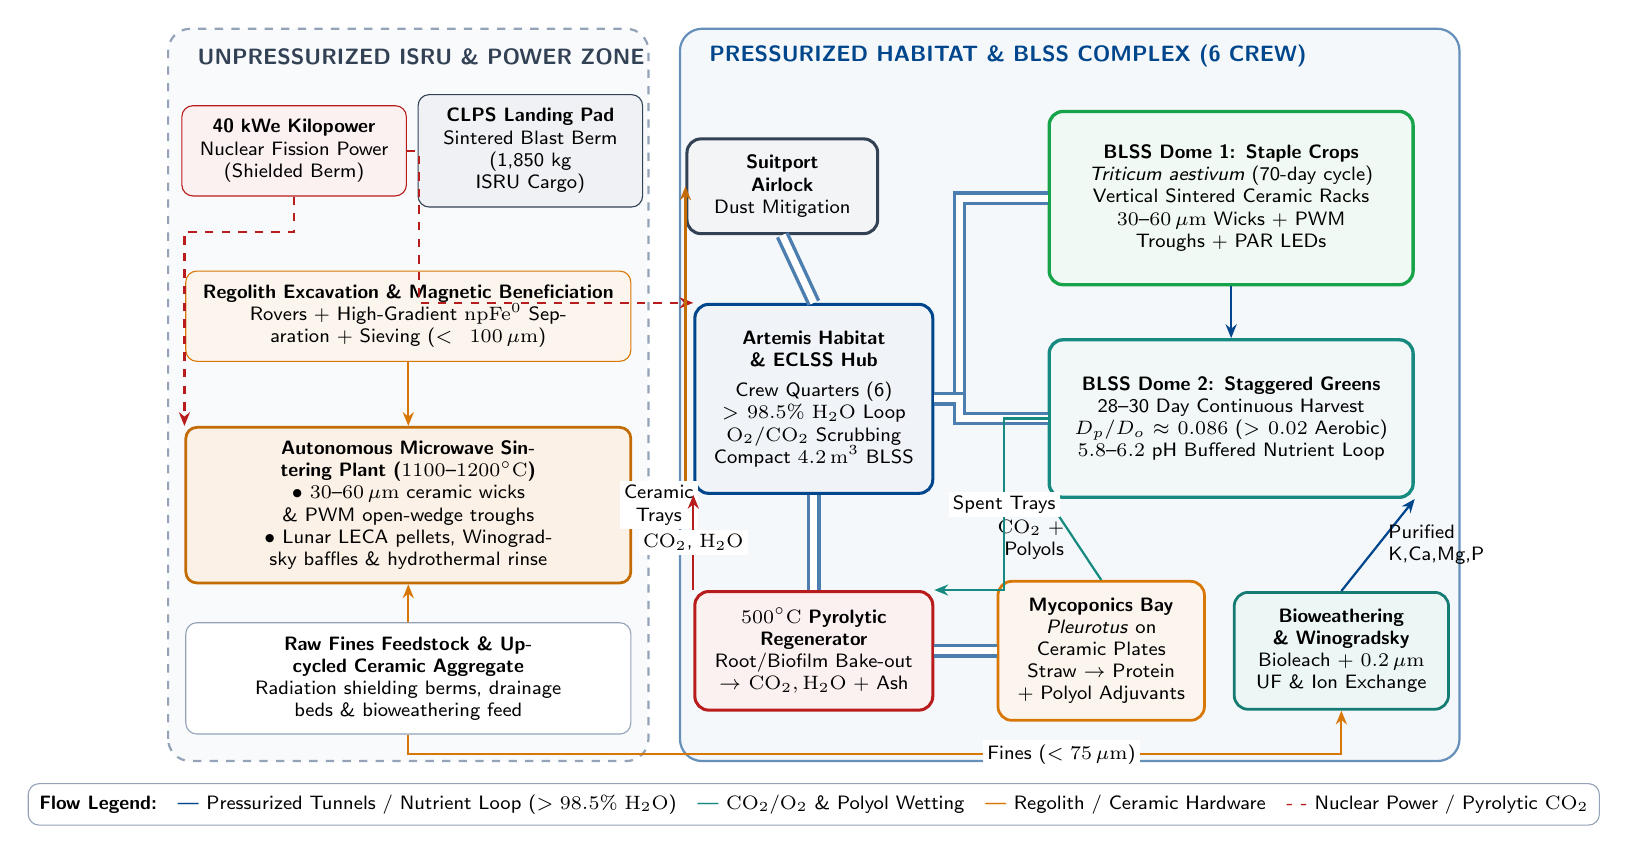
\begin{tikzpicture}[
    font=\sffamily\footnotesize,
    zonetitle/.style={
        font=\sffamily\bfseries\small,
        anchor=west
    },
    modbox/.style={
        draw=slateborder,
        rounded corners=4pt,
        fill=white,
        inner sep=5pt,
        align=center,
        font=\sffamily\scriptsize
    },
    pressbox/.style={
        draw=coseblue,
        line width=1.1pt,
        rounded corners=5pt,
        fill=white,
        inner sep=6pt,
        align=center,
        font=\sffamily\scriptsize
    },
    flow/.style={
        -{Stealth[length=5pt,width=4pt]},
        thick
    },
    tunnel/.style={
        draw=coseblue!70,
        line width=5pt
    },
    tunnelinner/.style={
        draw=white,
        line width=2.5pt
    }
]

% =========================================================================
% BACKGROUND ZONES (UNPRESSURIZED ISRU vs PRESSURIZED BLSS HABITAT)
% =========================================================================
% Left: Unpressurized Surface & ISRU Zone
\begin{scope}[on background layer]
    \fill[slatebg, rounded corners=8pt] (-8.2, -4.6) rectangle (-2.1, 4.7);
    \draw[slateborder, dashed, thick, rounded corners=8pt] (-8.2, -4.6) rectangle (-2.1, 4.7);

    % Right: Pressurized Habitat & Closed-Loop BLSS Complex
    \fill[coseblue!4, rounded corners=8pt] (-1.7, -4.6) rectangle (8.2, 4.7);
    \draw[coseblue!60, thick, rounded corners=8pt] (-1.7, -4.6) rectangle (8.2, 4.7);
\end{scope}

\node[font=\sffamily\bfseries\footnotesize, text=slatetext, anchor=west] at (-7.95, 4.35) {UNPRESSURIZED ISRU \& POWER ZONE};
\node[font=\sffamily\bfseries\footnotesize, text=coseblue, anchor=west] at (-1.45, 4.35) {PRESSURIZED HABITAT \& BLSS COMPLEX (6 CREW)};

% =========================================================================
% LEFT ZONE: POWER, LANDING, EXCAVATION & SINTERING
% =========================================================================
% Kilopower FSP
\node[modbox, draw=cosered, fill=cosered!6, text width=2.5cm] (fsp) at (-6.6, 3.15) {
    \textbf{40 kWe Kilopower}\\
    Nuclear Fission Power\\(Shielded Berm)
};

% CLPS Landing Pad
\node[modbox, draw=slatetext, fill=slateborder!15, text width=2.5cm] (pad) at (-3.6, 3.15) {
    \textbf{CLPS Landing Pad}\\
    Sintered Blast Berm\\(1,850 kg ISRU Cargo)
};

% Excavation & Beneficiation
\node[modbox, draw=coseamber, fill=coseamber!7, text width=5.3cm] (excav) at (-5.15, 1.05) {
    \textbf{Regolith Excavation \& Magnetic Beneficiation}\\
    Rovers + High-Gradient $\mathrm{npFe}^0$ Separation + Sieving ($<100\,\mu\mathrm{m}$)
};

% Microwave Sintering Plant
\node[modbox, draw=coseamber!90!black, line width=1pt, fill=coseamber!10, text width=5.3cm] (sinter) at (-5.15, -1.35) {
    \textbf{Autonomous Microwave Sintering Plant ($1100\text{--}1200^\circ\mathrm{C}$)}\\
    $\bullet$ $30\text{--}60\,\mu\mathrm{m}$ ceramic wicks \& PWM open-wedge troughs\\
    $\bullet$ Lunar LECA pellets, Winogradsky baffles \& hydrothermal rinse
};

% Regolith Stockpile / Berm
\node[modbox, draw=slateborder, fill=white, text width=5.3cm] (berm) at (-5.15, -3.55) {
    \textbf{Raw Fines Feedstock \& Upcycled Ceramic Aggregate}\\
    Radiation shielding berms, drainage beds \& bioweathering feed
};

% =========================================================================
% CENTER: AIRLOCK, HABITAT & ECLSS CORE
% =========================================================================
% Dust-lock Airlock
\node[pressbox, draw=slatetext, fill=slateborder!12, text width=2.0cm] (airlock) at (-0.4, 2.7) {
    \textbf{Suitport}\\
    \textbf{Airlock}\\
    Dust Mitigation
};

% Artemis Habitat Core
\node[pressbox, fill=coseblue!6, text width=2.6cm, minimum height=2.4cm] (hab) at (0.0, 0.0) {
    \textbf{Artemis Habitat}\\
    \textbf{\& ECLSS Hub}\\[3pt]
    Crew Quarters (6)\\
    $>98.5\%$ $\mathrm{H}_2\mathrm{O}$ Loop\\
    $\mathrm{O}_2/\mathrm{CO}_2$ Scrubbing\\
    Compact $4.2\,\mathrm{m}^3$ BLSS
};

% Pyrolytic Regenerator
\node[pressbox, draw=cosered, fill=cosered!6, text width=2.6cm] (pyro) at (0.0, -3.2) {
    \textbf{$500^\circ\mathrm{C}$ Pyrolytic}\\
    \textbf{Regenerator}\\
    Root/Biofilm Bake-out\\
    $\to \mathrm{CO}_2, \mathrm{H}_2\mathrm{O}$ + Ash
};

% =========================================================================
% RIGHT: BLSS GREENHOUSE DOMES, MYCOPONICS & BIOWEATHERING
% =========================================================================
% Dome 1: Primary Carbohydrate Crop Dome
\node[pressbox, draw=cosegreen, line width=1.2pt, fill=cosegreen!6, text width=4.2cm, minimum height=2.2cm] (dome1) at (5.3, 2.55) {
    \textbf{BLSS Dome 1: Staple Crops}\\
    \textit{Triticum aestivum} (70-day cycle)\\
    Vertical Sintered Ceramic Racks\\
    $30\text{--}60\,\mu\mathrm{m}$ Wicks + PWM Troughs + PAR LEDs
};

% Dome 2: Staggered Greens & Salad Dome
\node[pressbox, draw=coseteal, line width=1.2pt, fill=coseteal!6, text width=4.2cm, minimum height=2.0cm] (dome2) at (5.3, -0.25) {
    \textbf{BLSS Dome 2: Staggered Greens}\\
    28--30 Day Continuous Harvest\\
    $D_p/D_o \approx 0.086$ ($>0.02$ Aerobic)\\
    $5.8\text{--}6.2$ pH Buffered Nutrient Loop
};

% Mycoponics & Bioweathering Bay
\node[pressbox, draw=coseamber, line width=1pt, fill=coseamber!7, text width=2.2cm] (myco) at (3.65, -3.2) {
    \textbf{Mycoponics Bay}\\
    \textit{Pleurotus} on\\Ceramic Plates\\
    Straw $\to$ Protein\\+ Polyol Adjuvants
};

\node[pressbox, draw=coseteal!90!black, line width=1pt, fill=coseteal!8, text width=2.3cm] (biow) at (6.7, -3.2) {
    \textbf{Bioweathering}\\
    \textbf{\& Winogradsky}\\
    Bioleach + $0.2\,\mu\mathrm{m}$\\UF \& Ion Exchange
};

% =========================================================================
% PRESSURIZED TRANSFER TUNNELS
% =========================================================================
\draw[tunnel] (airlock.south) -- (hab.north);
\draw[tunnelinner] (airlock.south) -- (hab.north);

\draw[tunnel] (hab.east) -- (1.85, 0) |- (dome1.west);
\draw[tunnelinner] (hab.east) -- (1.85, 0) |- (dome1.west);

\draw[tunnel] (hab.east) -- (1.85, 0) |- (dome2.west);
\draw[tunnelinner] (hab.east) -- (1.85, 0) |- (dome2.west);

\draw[tunnel] (hab.south) -- (pyro.north);
\draw[tunnelinner] (hab.south) -- (pyro.north);

\draw[tunnel] (pyro.east) -- (myco.west);
\draw[tunnelinner] (pyro.east) -- (myco.west);

% =========================================================================
% MATERIAL, FLUID, GAS & POWER FLOWS
% =========================================================================
% Power from Kilopower
\draw[flow, draw=cosered, dashed] (fsp.south) -- ++(0, -0.45) -| (sinter.north west);
\draw[flow, draw=cosered, dashed] (fsp.east) -- ++(0.15, 0) |- (hab.north west);

% Regolith feedstock to Sintering & Bioweathering
\draw[flow, draw=coseamber] (excav.south) -- (sinter.north);
\draw[flow, draw=coseamber] (berm.north) -- (sinter.south);
\draw[flow, draw=coseamber] (berm.south) -- ++(0, -0.25) -| (biow.south) node[pos=0.35, fill=white, inner sep=1.5pt, font=\sffamily\scriptsize] {Fines ($<75\,\mu\mathrm{m}$)};

% Sintered trays from Plant to Airlock/Domes
\draw[flow, draw=coseamber!90!black] (sinter.east) -| (airlock.west) node[pos=0.25, fill=white, inner sep=1.5pt, font=\sffamily\scriptsize, align=center] {Ceramic\\Trays};

% Closed-loop Water & Nutrients (Blue)
\draw[flow, draw=coseblue] (biow.north) -- (dome2.south east) node[midway, right, font=\sffamily\scriptsize, align=left] {Purified\\K,Ca,Mg,P};
\draw[flow, draw=coseblue] (dome1.south) -- (dome2.north);

% Gas / Polyols / Biomass (Teal)
\draw[flow, draw=coseteal] (myco.north) -- (dome2.south west) node[midway, left, font=\sffamily\scriptsize, align=right] {$\mathrm{CO}_2$ +\\Polyols};
\draw[flow, draw=coseteal] (dome2.west) -- ++(-0.55, 0) |- (pyro.north east) node[pos=0.25, fill=white, inner sep=1.5pt, font=\sffamily\scriptsize] {Spent Trays};

% Pyrolytic CO2/H2O return
\draw[flow, draw=cosered] (pyro.north west) -- (hab.south west) node[midway, fill=white, inner sep=1.5pt, font=\sffamily\scriptsize, align=center] {$\mathrm{CO}_2$, $\mathrm{H}_2\mathrm{O}$};

% =========================================================================
% LEGEND BAR AT BOTTOM
% =========================================================================
\node[draw=slateborder, fill=white, rounded corners=4pt, inner sep=4pt, font=\sffamily\scriptsize] at (0.0, -5.15) {
    \textbf{Flow Legend:}\quad
    \textcolor{coseblue}{\textbf{---}} Pressurized Tunnels / Nutrient Loop ($>98.5\%$ $\mathrm{H}_2\mathrm{O}$)\quad
    \textcolor{coseteal}{\textbf{---}} $\mathrm{CO}_2$/$\mathrm{O}_2$ \& Polyol Wetting\quad
    \textcolor{coseamber}{\textbf{---}} Regolith / Ceramic Hardware\quad
    \textcolor{cosered}{\textbf{- -}} Nuclear Power / Pyrolytic $\mathrm{CO}_2$
};

\end{tikzpicture}
\end{document}
